\chapter{Softwareumsetzung}
\label{cha:Software}

Mit Hilfe des in Kapitel \ref{sec:Kamera} beschriebenen Kameramoduls müssen verschiedene Aufgaben aus dem Bereich der Bildverarbeitung bewältigt werden. 

\section{Wahl der Bildverarbeitungsbibliothek}

Die Umsetzung der zu bewältigenden Aufgaben kann durch die Wahl einer geeigneten Bildverarbeitungsbibliothek deutlich vereinfacht werden. Wichtige Kriterien für die Wahl der Bibliothek sind unter anderem Funktionsumfang, Dokumentation und aktivität der Community.

\subsection{LibCCV}

LibCCV \cite{libccv} ist eine open-source Bildverarbeitungsbilbiothek, die viele bekannte Algorithmen implementiert. LibCCV steht unter einer BSD-Clause-3-Lizenz und kann somit für eine Studienarbeit problemlos unbegrenzt verwendet werden. Die Bibliothek ist größtenteils in C++ verfasst und somit potenziell auf einem Android-Smartphone verwendet werden. Die Verwendung auf dem Smartphone wird jedoch nicht offiziell unterstützt und kann potenziell weitere Schwierigkeiten mit sich bringen.

\subsection{Imagemagick}

Bei Imagemagick \cite{imagemagick} handelt es sich um eine Bildverarbeitungsbibliothek, welche sehr viele Algorithmen bereits implementiert hat. Algorithmen zur Objekterkennung müssten jedoch vollständig selbst implementiert werden, was zu einem großen zusätzlichen Aufwand führen kann. Imagemagick wird unter der Apache 2.0 Lizenz vertrieben.

\subsection{OpenCV}
\label{subsec:opencv}

OpenCV \cite{opencv_library, bradski2008learning} stellt eine der größten Open-Source-Bibliotheken für Bildverarbeitung da. Die Bibliothek hat einen starken Focus auf Echtzeitverarbeitung und wird daher auch in vielen Projekten im Bereich der Robotik verwendet. OpenCV hat eine große aktive Community, wodurch eventuelle Fragen und Probleme schnell beantwortet werden können. Zusätzlich bietet OpenCV eine offizielle Verison für Android und eignet sich somit ideal für diese Studienarbeit.


\section{Algorithmus zur Objekterkennung}

Aufgabe des Roboters, ist es Gegenstände in einem Raum mit Hilfe von Kamerabildern zu erkennen. Folglich spielt die Objekterkennung eine große Rolle.

\subsection{Farbbasierte Objekterkennung}
Einen einfachen Ansatz der Objekterkennung unter Verwendung von Methoden der in \ref{subsec:opencv} beschriebenen Bibliothek OpenCV stellt eine farbbasierte Objekterkennung dar. Hierfür wird das Kamerabild zunächst vom RGB-Format [ZITAT EINFÜGEN] in das HSV-Format [ZITAT] konvertiert. Dies wird durchgeführt, da das HSV-Format unempfindlicher gegen Veränderungen in der Beleuchtung ist als das RGB-Format. Abbildung \ref{fig:ColorModels} zeigt die Aufteilung eines Bildes in die verschiedenen Kanäle.

\begin{figure}[h]
\centering
\includegraphics[width=\textwidth]{Bilder/Software/ColormodelsAll}
\caption{Beispiel einer Aufspaltung in RGB-Kanäle (links) und HSV-Kanäle (rechts)}
\label{fig:ColorModels}
\end{figure}

Wie in Abbildung \ref{fig:ColorModels} zu sehen ist, eignet sich vor allem der Saturation-Kanal des Bildes um farbige Objekte zu erkennen, da dieser hohe Werte annimmt wenn die Farbintensität hoch ist. Zuletzt erfolgt eine Binarisierung mit einem empirisch ermittelten Schwellwert von 50. Dies ist notwendig, da die, in der OpenCV-Bibliothek implementierte, Methode von Suzuki und Abe \cite{suzuki1985topological} zur Segmentierung von Objekten ein Binärbild erwartet. Aus dem in Abbildung \ref{fig:ColorModels} dargestellten Beispiel entsteht nach der Binarisierung schließlich Abbildung \ref{fig:BinarizedColorModels}. Der Algorithmus zur Segmentierung erkennt daraus drei Objekte und zeichnet ihren Konturen, wie in Abbildung \ref{fig:SegmentedColorModels} ersichtlich, ein.

\begin{figure}[h]
\centering

\includegraphics[width=\textwidth/2]{Bilder/Software/ColormodelsBinarized}
\caption{Beispiel der Binarisierung des Sättigungskanals}
\label{fig:BinarizedColorModels}
\end{figure}
\begin{figure}[h]
\centering
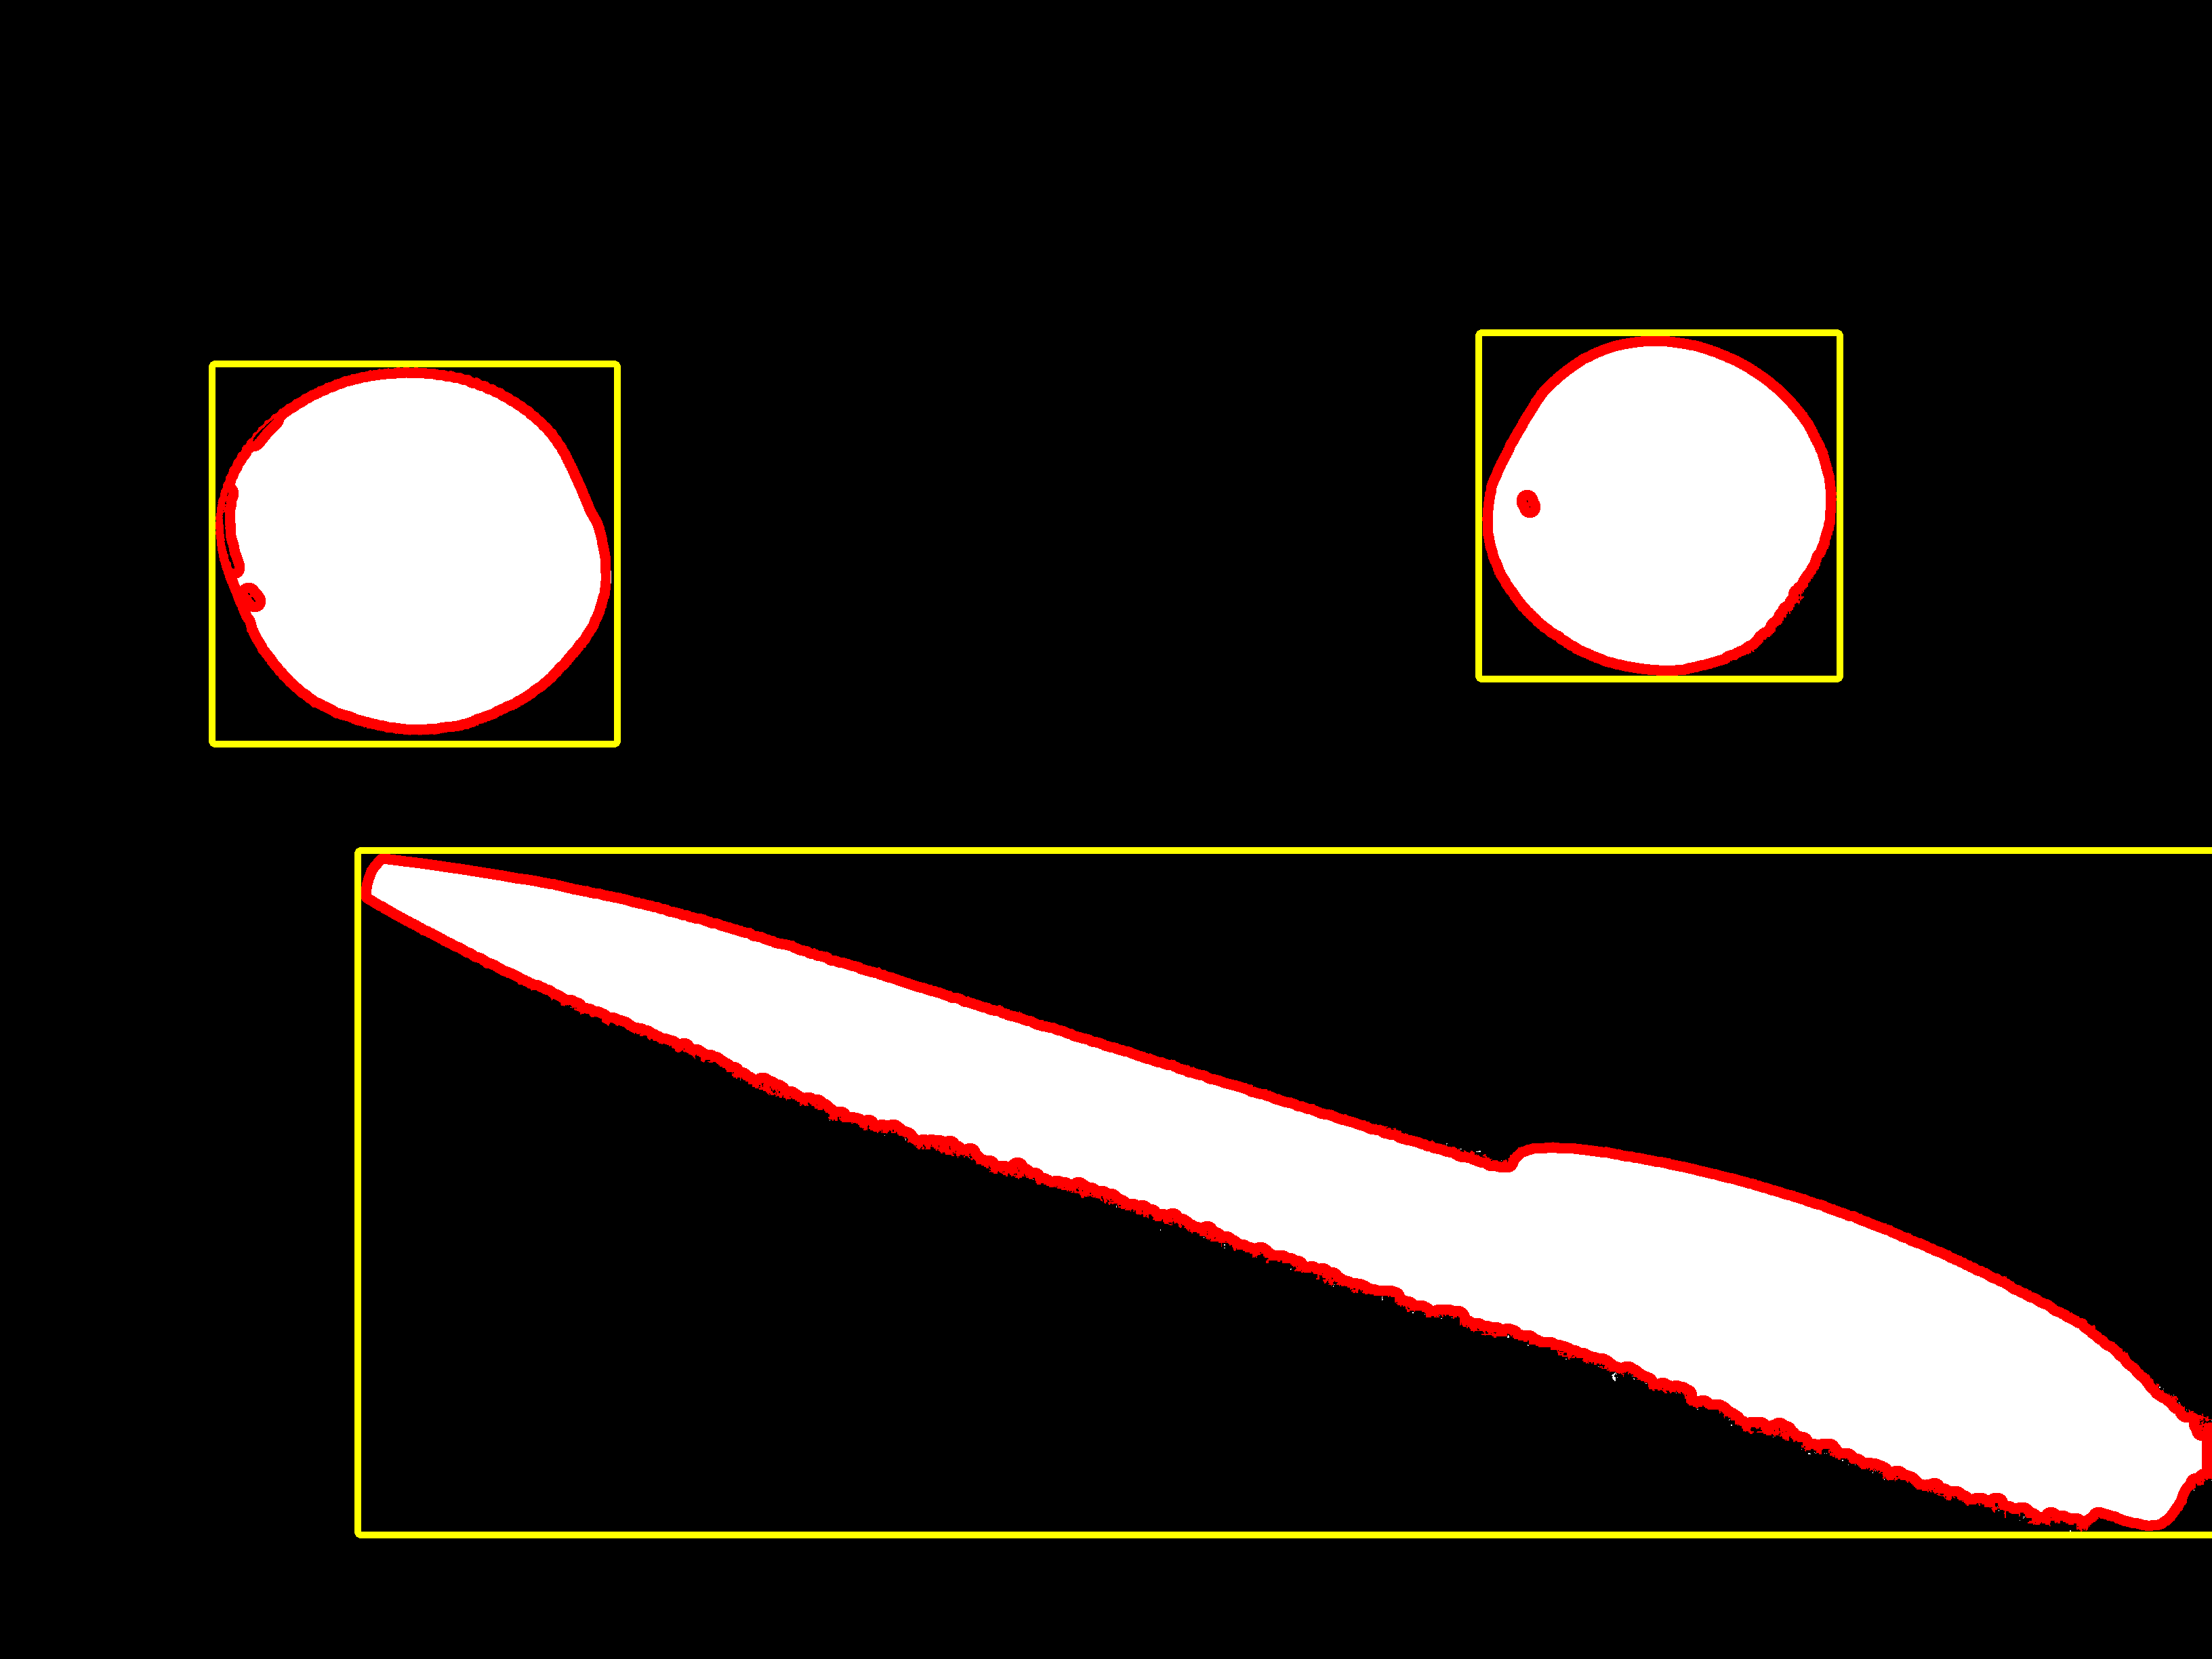
\includegraphics[width=\textwidth/2]{Bilder/Software/ColormodelsSegmentated}
\caption{Beispiel einer Segmentierung des binarisierten Sättigungskanals}
\label{fig:SegmentedColorModels}
\end{figure}


\section{Entfernungsschätzung}
\subsection{Stereo-Kamerabasiert}
\subsection{Mono-Kamerabasiert}
\subsection{Ultraschallbasiert}

\section{Raumerkennung}
\subsection{Kameragestützt}
\subsection{Streckenbasiert}
Über gefahrene Strecke
\subsection{Kombination unterschiedlicher Sensordaten}


\section{Zielzonenerkennung}


\section{Hauptschleife}

Arbeitszustände
\begin{enumerate}
\item{Objekt suchen}
\item{Objekt ansteuern}
\item{Objekt aufnehmen}
\item{Objekt kategorisieren}
\item{Zielbereich suchen}
\item{Zielbereich ansteuern}
\item{Objekt ablegen}
\end{enumerate}

[INSERT ZUSTANDSÜBERGANGSDIAGRAMM]

